%%%%%%%%%%%%%%%%%%%%%%%%%%%%%%%%%%%%%%%%%%%%%%%%%%%%%%%%%%%%
%%%%%%%%%%%%%%%%%%%%%%%%%%%%%%%%%%%%%%%%%%%%%%%%%%%%%%%%%%%%
%%%%%%%%%%%%%%%%%%%%%%%%%%%%%%%%%%%%%%%%%%%%%%%%%%%%%%%%%%%%
\section{Algebraic Formulation}
%%%%%%%%%%%%%%%%%%%%%%%%%%%%%%%%%%%%%%%%%%%%%%%%%%%%%%%%%%%%
%%%%%%%%%%%%%%%%%%%%%%%%%%%%%%%%%%%%%%%%%%%%%%%%%%%%%%%%%%%%
%%%%%%%%%%%%%%%%%%%%%%%%%%%%%%%%%%%%%%%%%%%%%%%%%%%%%%%%%%%%

\subsection{Solution of the Unconstrained Problem}

\paragraph{Unconstrained Problem in Original Basis}

\begin{frame}
\frametitle<presentation>{Unconstrained Problem in Original Basis}
We recall the unconstrained problem in weighted residual form:
\begin{equation}
u_h\in U_h\ : \qquad r_h(u_h,v) = 0 \qquad \forall
v\in V_h .
\end{equation}

Solving it in the original basis
reduces to the solution of a nonlinear algebraic problem:
\begin{equation}
\begin{split}
\mathbf{u}\in\mathbf{U} : \qquad
& r_h\left(\text{FE}_{\Phi_{U_h}}(\mathbf{u}),\psi_i\right) = 0, \quad
i\in\mathcal{I}_{V_h} \\
\Leftrightarrow \  & \mathcal{R}(\mathbf{u}) = \mathbf{0}
\end{split}
\end{equation}
where we introduced the nonlinear residual map $\mathcal{R} :
\mathbf{U} = \mathbb{K}^{\mathcal{I}_{V_h}} \to \mathbb{K}^{\mathcal{I}_{V_h}}$ which is defined as 
\begin{equation}
\left(
\mathcal{R}(\mathbf{u})\right)_i =
r_h(\text{FE}_{U_h}(\mathbf{u}),\psi_i).
\end{equation}
$\Phi_{V_h} = \{\psi_i\,|\, i\in\mathcal{I}_{V_h}\}$ is the basis of $V_h$.  
\end{frame}

\paragraph{Unconstrained Problem in Transformed Basis}

\begin{frame}
\frametitle<presentation>{Unconstrained Problem in Transformed Basis}
We may also solve the unconstrained problem 
in the transformed basis for trial and test space:
\begin{equation}\label{Eq:TransformedUnconstrainedProblem}
\begin{split}
\mathbf{u}'\in\mathbf{U}' : \qquad 
& r_h\left(\text{FE}_{\Phi'_{U_h}}(\mathbf{u}'),\psi_i'\right) = 0, \quad
i\in\mathcal{I}_{V_h}\\
\Leftrightarrow \  &
r_h\left(\text{FE}_{\Phi_{U_h}}(\mathbf{T}^T_{U_h}\mathbf{u}'),
\sum_{j\in\mathcal{I}_{V_h}}\left(\mathbf{T}_{V_h}\right)_{i,j}\psi_j\right) = 0, \quad
i\in\mathcal{I}_{V_h}\\
\Leftrightarrow \  &
\sum_{j\in\mathcal{I}_{V_h}} \left(\mathbf{T}_{V_h}\right)_{i,j} 
r_h\left(\text{FE}_{\Phi_{U_h}}(\mathbf{T}^T_{U_h}\mathbf{u}'),
\psi_j\right) = 0, \quad
i\in\mathcal{I}_{V_h}\\
\Leftrightarrow \  &
\mathbf{T}_{V_h} \mathcal{R}\left(\mathbf{T}^T_{U_h}\mathbf{u}'\right)
= \mathbf{0} .
\end{split}
\end{equation}
Used linearity of residual form with respect to the second argument.

Requires simple matrix multiplication.
\end{frame}

\paragraph{Newton solver}

Use Newton's method to solve the algebraic problem.

\begin{frame}<article>
\frametitle<presentation>{Newton Solver}
Let a current iterate $\mathbf{u}_k'$ be given. 

We seek an update $\mathbf{z}'_k$ such that $\mathbf{u}'_{k+1} = \mathbf{u}_k'
+ \mathbf{z}'_k$ and linearize:
\begin{equation*}
\mathbf{T}_{V_h}\mathcal{R}\left(\mathbf{T}^T_{U_h}\mathbf{u}'_{k+1}\right) \approx 
\mathbf{T}_{V_h}\mathcal{R}\left(\mathbf{T}^T_{U_h}\mathbf{u}'_{k}\right) +
\mathbf{T}_{V_h}\nabla\mathcal{R}\left(\mathbf{T}^T_{U_h}\mathbf{u}'_{k}\right) 
\mathbf{T}^T_{U_h} \mathbf{z}'_{k} = \mathbf{0} .
\end{equation*}

A linear system for the update is 
\begin{equation}\label{eq:UnconstrainedUpdate}
\mathbf{T}_{V_h}\nabla\mathcal{R}\left(\mathbf{T}^T_{U_h}\mathbf{u}'_{k}\right) 
\mathbf{T}^T_{U_h} \mathbf{z}'_{k} = -
\mathbf{T}_{V_h}\mathcal{R}\left(\mathbf{T}^T_{U_h}\mathbf{u}'_{k}\right) .
\end{equation}

$\nabla\mathcal{R}\left(\mathbf{u}_{k}\right)$ denotes the
Jacobian matrix of the map $\mathcal{R}$. 

Multiplying the update equation with $\mathbf{T}^T_{U_h}$ from the left yields
\begin{equation}\label{eq:OriginalUpdate}
\mathbf{T}^T_{U_h}\mathbf{u}'_{k+1} = \mathbf{T}^T_{U_h}\mathbf{u}_k' +
\mathbf{T}^T_{U_h}\mathbf{z}'_k .
\end{equation}

Setting $\mathbf{u}_{k} := \mathbf{T}^T_{U_h}\mathbf{u}_k'$ allows us
now to write the Newton scheme with respect to the original basis.
\end{frame}


\begin{frame}
\frametitle<presentation>{Newton Solver (Contd.)}
\begin{Alg}[Newton's method for unconstrained problem]
Given the initial guess $\mathbf{u}_{0}$ iterate until convergence
\begin{enumerate}[i)]
\item Compute residual:
  $\mathbf{r}_k=\mathcal{R}\left(\mathbf{u}_{k}\right)$.
\item Transform residual: $\mathbf{r}_k' = \mathbf{T}_{V_h}
  \mathbf{r}_k$.
\item Solve update equation:
  $\mathbf{T}_{V_h}\nabla\mathcal{R}\left(\mathbf{u}_{k}\right)  
\mathbf{T}^T_{U_h} \mathbf{z}'_{k} =  \mathbf{r}_k'$.
\item Transform update: $\mathbf{z}_{k} =
  \mathbf{T}^T_{U_h}\mathbf{z}'_k$.
\item Update: $\mathbf{u}_{k+1} = \mathbf{u}_k
- \mathbf{z}_k$. \hfill$\square$
\end{enumerate}
\end{Alg}

Two applications of the basis transformation, for the
residual and the update, are necessary in steps ii) and iv).

These transformations are cheap due to the structure of the
transformation.

In step (iii) the \textit{transformed}
Jacobian system is required.

\textit{All these transformations are done generically by PDELab}!
\end{frame}

\subsection{Solution of Constrained Problem}

We now turn to the constrained problem.

\paragraph{Reformulation in unconstrained space}

\begin{frame}<article>
\frametitle<presentation>{Reformulation in unconstrained space}
We recall the constrained problem in weighted residual form:
\begin{equation}\label{Eq:ConstrainedProblem}
u_h\in w_h + \tilde{U}_h\ : \qquad r_h(u_h,v) = 0 \quad \forall
v\in \tilde{V}_h .
\end{equation}

This problem can be reformulated in the unconstrained space by adding
a constrained equation:
\begin{Prp}
Let $P_h : U_h \to \tilde{U}_h$ be a projection (i.~e.~$P_h^2 = P_h$)
and assume that the affine shift is such that $P_h w_h = 0$. Then 
\begin{equation}\label{Eq:ConstrainedProblemReformII}
u_h\in U_h\ : \qquad \left\{\begin{array}{ll}
r_h(u_h,v) = 0 \quad \forall v\in \tilde{V}_h\\
(I-P_h)u_h = w_h
\end{array}\right. 
\end{equation}
is equivalent to \eqref{Eq:ConstrainedProblem}.

\mode<article>{
\textit{Proof}. Assume that \eqref{Eq:ConstrainedProblem} holds and
$P_h w_h = 0$. Since $u_h$ solves \eqref{Eq:ConstrainedProblem}
the first equation in \eqref{Eq:ConstrainedProblemReformII} clearly holds.
Moreover, we have $u_h = w_h + \tilde{u}_h$ with $\tilde{u}_h\in
\tilde{U}_h$ which allows us to write $u_h = w_h + P_h v_h$ for some
$v_h\in U_h$. When we can prove that $v_h=u_h$ we obtain the desired
$(I-P_h)u_h = w_h$. We now show that $v_h=u_h$:
Applying $P_h$ to both sides of the identity $u_h = w_h + P_h v_h$ yields
$P_h u_h = P_h w_h + P_h^2 v_h$. Using $P_h w_h = 0$ and $P_h^2 = P_h$
yields $P_h u_h = P_h v_h$. Thus we may identify $v_h$ and $u_h$ as
$v_h$ was arbitrary.\\
Assume now that \eqref{Eq:ConstrainedProblemReformII} holds. The first
equation of \eqref{Eq:ConstrainedProblemReformII} is the same as 
\eqref{Eq:ConstrainedProblem}. From the
second equation we conclude $u_h = w_h + P_h u_h$, i.~e.~ $u_h\in w_h
+ \tilde{U}_h$.} \hfill$\square$
\end{Prp}
\end{frame}

\paragraph{Reformulated Problem in Coefficient Space} 

We now seek to solve problem
\eqref{Eq:ConstrainedProblemReformII} in coefficient space. 

\begin{frame}<article>
\frametitle<presentation>{Reformulated Problem in Coefficient Space}
The projection $P_h$ is taken from the follwing commutative diagram:
\begin{equation*}
\begin{CD}
U_h @>{P_h = \text{FE}_{\Phi'_{U_h}}
\mathbf{R}^T_{\tilde{\mathbf{U}}',\mathbf{U}'}
\mathbf{R}_{\tilde{\mathbf{U}}',\mathbf{U}'} 
\text{FE}_{\Phi'_{U_h}}^{-1}}>> \tilde{U}_h\\
@A{\text{FE}_{\Phi'_{U_h}}}AA @AA{\text{FE}_{\Phi'_{U_h}}
\mathbf{R}^T_{\tilde{\mathbf{U}}'\mathbf{U}'}}A\\
\mathbf{U}' @>{\qquad\mathbf{R}_{\tilde{\mathbf{U}}',\mathbf{U}'}\qquad}>> \tilde{\mathbf{U}}' 
\end{CD}
\end{equation*}

\begin{Prp}
Using this definition of $P_h$ the reformulated constrained
problem \eqref{Eq:ConstrainedProblemReformII} in coefficient space reads
\begin{equation}\label{Eq:ConstrainedProblemInCoefficientSpace}
\mathbf{u}'\in\mathbf{U}' : \qquad \left\{\begin{array}{rcl}
\mathbf{S}_{\tilde{\mathbf{V}}'}
\mathcal{R}\left(\mathbf{T}^T_{U_h}\mathbf{u}'\right)
& = & \mathbf{0}\\
\mathbf{R}_{\bar{\mathbf{U}}',\mathbf{U}'} \mathbf{u}' & = & \mathbf{w}'
\end{array}\right.
\end{equation}
with $\mathbf{S}_{\tilde{\mathbf{V}}'}=\mathbf{R}_{\tilde{\mathbf{V}}',\mathbf{V}'} +
\mathbf{T}_{\tilde{V}_h,\bar{V}_h}\mathbf{R}_{\bar{\mathbf{V}}',\mathbf{V}'}$
and $w_h =
FE_{\Phi_{U_h}'}(\mathbf{R}_{\bar{\mathbf{U}}',\mathbf{U}'}^T\mathbf{w}')$.
\hfill$\square$
\end{Prp}
\end{frame}

The idea in this formulation is that with respect to the transformed
basis the affine shift (for Dirichlet boundary conditions) can be
``encoded'' in the constrained degrees of freedom
$\mathbf{R}_{\bar{\mathbf{U}}',\mathbf{U}'} \mathbf{u}'$. This is
possible because the subspace $\tilde{U}_h$ is the image
of the unconstrained degrees of freedom
$\mathbf{R}_{\tilde{\mathbf{U}}',\mathbf{U}'} \mathbf{u}'$ 
and the decomposition is orthogonal
(i.~e.~$\mathbf{R}^T_{\bar{\mathbf{U}}',\mathbf{U}'}
\mathbf{R}_{\bar{\mathbf{U}}',\mathbf{U}'}$ and
$\mathbf{R}^T_{\tilde{\mathbf{U}}',\mathbf{U}'}
\mathbf{R}_{\tilde{\mathbf{U}}',\mathbf{U}'}$ are orthogonal
projections). 


\begin{frame}<article>
\frametitle<presentation>{Proof of Proposition}
The second equation is seen as follows:
\begin{equation}\label{Eq:SideConditionCoefficient}
\begin{split}
&(I-P_h) u_h = w_h \\
\Leftrightarrow \quad & 
\left(\text{FE}_{\Phi'_{U_h}}\text{FE}_{\Phi'_{U_h}}^{-1}
- \text{FE}_{\Phi'_{U_h}}
\mathbf{R}^T_{\tilde{\mathbf{U}}',\mathbf{U}'}
\mathbf{R}_{\tilde{\mathbf{U}}',\mathbf{U}'} 
\text{FE}_{\Phi'_{U_h}}^{-1}\right)\text{FE}_{\Phi'_{U_h}}\mathbf{u}'
= \text{FE}_{\Phi'_{U_h}}
\mathbf{R}^T_{\bar{\mathbf{U}}',\mathbf{U}'} \mathbf{w}'\\
\Leftrightarrow \quad &
\left( \mathbf{I} - \mathbf{R}^T_{\tilde{\mathbf{U}}',\mathbf{U}'}
\mathbf{R}_{\tilde{\mathbf{U}}',\mathbf{U}'}\right) \mathbf{u}' =
\mathbf{R}^T_{\bar{\mathbf{U}}',\mathbf{U}'} \mathbf{w}' \\
\Leftrightarrow \quad &
\mathbf{R}^T_{\bar{\mathbf{U}}',\mathbf{U}'}
\mathbf{R}_{\bar{\mathbf{U}}',\mathbf{U}'} \mathbf{u}' =
\mathbf{R}^T_{\bar{\mathbf{U}}',\mathbf{U}'} \mathbf{w}'\\
\Leftrightarrow \quad &
\mathbf{R}_{\bar{\mathbf{U}}',\mathbf{U}'} \mathbf{u}' = \mathbf{w}' .
\end{split}
\end{equation}
\end{frame}

\begin{frame}<article>
\frametitle<presentation>{Proof of Proposition (Contd.)}
For the first equation in \eqref{Eq:ConstrainedProblemReformII} 
we proceed as in \eqref{Eq:TransformedUnconstrainedProblem}
\begin{equation}\label{Eq:TransformedConstrainedProblem2}
\begin{split}
\mathbf{u}'\in\mathbf{U}' : \qquad 
& r_h\left(\text{FE}_{\Phi'_{U_h}}(\mathbf{u}'),\psi_i'\right) = 0, \quad
i\in\tilde{\mathcal{I}}_{V_h}\\
\Leftrightarrow \  &
r_h\left(\text{FE}_{\Phi_{U_h}}(\mathbf{T}^T_{U_h}\mathbf{u}'),
\sum_{j\in\mathcal{I}_{V_h}}\left(\mathbf{T}_{V_h}\right)_{i,j}\psi_j\right) = 0, \quad
i\in\tilde{\mathcal{I}}_{V_h}\\
\Leftrightarrow \  &
\sum_{j\in\mathcal{I}_{V_h}} \left(\mathbf{T}_{V_h}\right)_{i,j} 
r_h\left(\text{FE}_{\Phi_{U_h}}(\mathbf{T}^T_{U_h}\mathbf{u}'),
\psi_j\right) = 0, \quad
i\in\tilde{\mathcal{I}}_{V_h}\\
\Leftrightarrow \  &
\underbrace{\left(\mathbf{R}_{\tilde{\mathbf{V}}',\mathbf{V}'} +
\mathbf{T}_{\tilde{V}_h,\bar{V}_h}\mathbf{R}_{\bar{\mathbf{V}}',\mathbf{V}'}
\right)}_{\mathbf{S}_{\tilde{\mathbf{V}}'}}\mathcal{R}\left(\mathbf{T}^T_{U_h}\mathbf{u}'\right)=
\mathbf{S}_{\tilde{\mathbf{V}}'} \mathcal{R}\left(\mathbf{T}^T_{U_h}\mathbf{u}'\right)
= \mathbf{0} .
\end{split}
\end{equation}
Here we made use of the structure of the transformation
\eqref{Eq:StructureTransformation} in the final line.
\end{frame}


\paragraph{Newton's Method for Constrained Problem}

Newton's method applied to the constrained
problem \eqref{Eq:ConstrainedProblemInCoefficientSpace} is formulated
in the following alorithm.

\begin{frame}
\frametitle<presentation>{Newton's Method for Constrained Problem}
\begin{Alg}[Newton's method for constrained problem]\label{algo:ConstrainedNewton}
Let the initial guess $\mathbf{u}_{0}$ with
$\text{FE}_{\Phi_{U_h}}(\mathbf{u}_{0}) \in w_h + \tilde{U}_h$ be given. 
Iterate until convergence
\begin{enumerate}[i)]
\item Compute residual:
  $\mathbf{r}_k=\mathcal{R}\left(\mathbf{u}_{k}\right)$.
\item Transform residual: $\mathbf{r}_k' = \mathbf{S}_{\tilde{\mathbf{V}}'}
  \mathbf{r}_k$.
\item Solve update equation:
\begin{equation*}
\left(\begin{array}{cc}
\mathbf{S}_{\tilde{\mathbf{V}}'} \nabla
\mathcal{R}\left(\mathbf{T}^T_{U_h}\mathbf{u}_{k}'\right)
\mathbf{S}^T_{\tilde{\mathbf{U}}'} & \mathbf{0}\\
\mathbf{0} & \mathbf{I}
\end{array}\right) 
\left(\begin{array}{c}
\tilde{\mathbf{z}}_{k}'\\
\bar{\mathbf{z}}_{k}'
\end{array}\right) =
\left(\begin{array}{c}
\mathbf{r}_k'\\
\mathbf{0}
\end{array}\right) 
\end{equation*}
and set $\mathbf{z}'_{k} = \left(\begin{smallmatrix}
\tilde{\mathbf{z}}_{k}'\\ \bar{\mathbf{z}}_{k}'
\end{smallmatrix}\right)$.
\item Transform update: $\mathbf{z}_{k} =
  \mathbf{T}^T_{U_h}\mathbf{z}'_k$. (This is where interpolation to
  hanging nodes is done).
\item Update: $\mathbf{u}_{k+1} = \mathbf{u}_k
- \mathbf{z}_k$. \hfill$\square$
\end{enumerate}
\end{Alg}
\end{frame}


\begin{frame}<article>
\frametitle<presentation>{Constraint Equation in Newton's Method}
Let $\mathbf{u}_{k}'$ be given.  Seek update $\mathbf{z}_{k}'$ s.t.
$\mathbf{u}_{k+1}' = \mathbf{u}_{k}' + \mathbf{z}_{k}'$. 

Inserting $\mathbf{u}_{k+1}'$ into the second equation of
\eqref{Eq:ConstrainedProblemInCoefficientSpace} yields
\begin{equation}\label{Eq:SideCond}
\begin{split}
& \mathbf{R}_{\bar{\mathbf{U}}',\mathbf{U}'} \mathbf{u}_{k+1}'
= \mathbf{R}_{\bar{\mathbf{U}}',\mathbf{U}'} \mathbf{u}_{k}' +
\mathbf{R}_{\bar{\mathbf{U}}',\mathbf{U}'} \mathbf{z}_{k}'
 =  \bar{\mathbf{w}}'\\ 
\Leftrightarrow\qquad &
\mathbf{R}_{\bar{\mathbf{U}}',\mathbf{U}'} \mathbf{z}_{k}' = 
\bar{\mathbf{w}}' - \mathbf{R}_{\bar{\mathbf{U}}',\mathbf{U}'}
\mathbf{u}_{k}' = \mathbf{0}\\
\Leftrightarrow\qquad &
\bar{\mathbf{z}}_{k}' = \mathbf{0}
\end{split}
\end{equation}
where we introduced $\mathbf{z}_{k}' =
\mathbf{R}^T_{\bar{\mathbf{U}}',\mathbf{U}'}
\bar{\mathbf{z}}_{k}'$ and used $\mathbf{R}_{\bar{\mathbf{U}}',\mathbf{U}'}
\mathbf{R}^T_{\bar{\mathbf{U}}',\mathbf{U}'}=\mathbf{I}$. 
Note that the affine shift is not changed during the iteration:
\begin{equation}
\mathbf{R}_{\bar{\mathbf{U}}',\mathbf{U}'}\mathbf{u}_{k+1}' =
\mathbf{R}_{\bar{\mathbf{U}}',\mathbf{U}'} \mathbf{u}_{k}' +
\underbrace{\mathbf{R}_{\bar{\mathbf{U}}',\mathbf{U}'}
  \mathbf{z}_{k}'}_{= \mathbf{0}} =
\mathbf{R}_{\bar{\mathbf{U}}',\mathbf{U}'} \mathbf{u}_{k}' .
\end{equation}
Thus it is sufficient to satisfy the affine shift in the initial
guess $\mathbf{R}_{\bar{\mathbf{U}}',\mathbf{U}'} \mathbf{u}_{0}' =
\bar{\mathbf{w}}'$.
\end{frame}

\begin{frame}<article>
\frametitle<presentation>{Constraint Equation in Newton's Method (Contd.)}
Now insert  $\mathbf{u}_{k+1}'$ into the first equation of
\eqref{Eq:ConstrainedProblemInCoefficientSpace}:
\begin{equation}
\begin{split}
\mathbf{S}_{\tilde{\mathbf{V}}'}
&\mathcal{R}\left(\mathbf{T}^T_{U_h}\mathbf{u}_{k+1}'\right)
= \mathbf{S}_{\tilde{\mathbf{V}}'}
\mathcal{R}\left(\mathbf{T}^T_{U_h}\mathbf{u}_{k}' +
\mathbf{T}^T_{U_h}\mathbf{z}_{k}' \right)\\
&= \mathbf{S}_{\tilde{\mathbf{V}}'}
\mathcal{R}\left(\mathbf{T}^T_{U_h}\mathbf{u}_{k}' +
\mathbf{T}^T_{U_h} \left(\mathbf{R}^T_{\bar{\mathbf{U}}',\mathbf{U}'}
\underbrace{\mathbf{R}_{\bar{\mathbf{U}}',\mathbf{U}'}
  \mathbf{z}_{k}'}_{=\mathbf{0}, \text{ cf.\eqref{Eq:SideCond}}} +
\mathbf{R}^T_{\tilde{\mathbf{U}}',\mathbf{U}'} 
\mathbf{R}_{\tilde{\mathbf{U}}',\mathbf{U}'} \mathbf{z}_{k}' \right)
\right)\\
&= \mathbf{S}_{\tilde{\mathbf{V}}'}
\mathcal{R}\left(\mathbf{T}^T_{U_h}\mathbf{u}_{k}' +
\mathbf{T}^T_{U_h} \mathbf{R}^T_{\tilde{\mathbf{U}}',\mathbf{U}'} 
\mathbf{R}_{\tilde{\mathbf{U}}',\mathbf{U}'} \mathbf{z}_{k}' \right)\\
&= \mathbf{S}_{\tilde{\mathbf{V}}'}
\mathcal{R}\left(\mathbf{T}^T_{U_h}\mathbf{u}_{k}' +
\underbrace{\left(\mathbf{R}^T_{\tilde{\mathbf{U}}',\mathbf{U}'} +
\mathbf{R}^T_{\bar{\mathbf{U}}',\mathbf{U}'} \mathbf{T}^T_{\tilde{U}_h,\bar{U}_h}
\right)}_{=: \,\mathbf{S}^T_{\tilde{\mathbf{U}}'}}
\mathbf{R}_{\tilde{\mathbf{U}}',\mathbf{U}'} \mathbf{z}_{k}' 
\right) \\
&= 
\mathbf{S}_{\tilde{\mathbf{V}}'}
\mathcal{R}\left(\mathbf{T}^T_{U_h}\mathbf{u}_{k}' + 
\mathbf{S}^T_{\tilde{\mathbf{U}}'}
\mathbf{R}_{\tilde{\mathbf{U}}',\mathbf{U}'}
\mathbf{R}^T_{\tilde{\mathbf{U}}',\mathbf{U}'} \tilde{\mathbf{z}}_{k}'
\right)
=
\mathbf{S}_{\tilde{\mathbf{V}}'}
\mathcal{R}\left(\mathbf{T}^T_{U_h}\mathbf{u}_{k}' + 
\mathbf{S}^T_{\tilde{\mathbf{U}}'} \tilde{\mathbf{z}}_{k}'\right)
\end{split}
\end{equation}
where we introduced $\mathbf{z}_{k}' =
\mathbf{R}^T_{\tilde{\mathbf{U}}',\mathbf{U}'}
\tilde{\mathbf{z}}_{k}'$ and used $\mathbf{R}_{\tilde{\mathbf{U}}',\mathbf{U}'}
\mathbf{R}^T_{\tilde{\mathbf{U}}',\mathbf{U}'}=\mathbf{I}$. 
\end{frame}


\begin{frame}<article>
\frametitle<presentation>{Constraint Equation in Newton's Method (Contd.)}
Linearization now gives
\begin{equation*}
\mathbf{S}_{\tilde{\mathbf{V}}'}
\mathcal{R}\left(\mathbf{T}^T_{U_h}\mathbf{u}_{k}' + 
\mathbf{S}^T_{\tilde{\mathbf{U}}'} \tilde{\mathbf{z}}_{k}'\right)
\approx \mathbf{S}_{\tilde{\mathbf{V}}'}
\mathcal{R}\left(\mathbf{T}^T_{U_h}\mathbf{u}_{k}'\right) 
+ \mathbf{S}_{\tilde{\mathbf{V}}'} \nabla
\mathcal{R}\left(\mathbf{T}^T_{U_h}\mathbf{u}_{k}'\right)
\mathbf{S}^T_{\tilde{\mathbf{U}}'} \tilde{\mathbf{z}}_{k}' = \mathbf{0}.
\end{equation*}
Thus the equation for the update reads
\begin{equation*}
\mathbf{S}_{\tilde{\mathbf{V}}'} \nabla
\mathcal{R}\left(\mathbf{T}^T_{U_h}\mathbf{u}_{k}'\right)
\mathbf{S}^T_{\tilde{\mathbf{U}}'} \tilde{\mathbf{z}}_{k}'
= - \mathbf{S}_{\tilde{\mathbf{V}}'}
\mathcal{R}\left(\mathbf{T}^T_{U_h}\mathbf{u}_{k}'\right) .
\end{equation*}
\end{frame}

\cleardoublepage

%%%%%%%%%%%%%%%%%%%%%%%%%%%%%%%%%%%%%%%%%%%%%%%%%%%%%%%%%%%%
%%%%%%%%%%%%%%%%%%%%%%%%%%%%%%%%%%%%%%%%%%%%%%%%%%%%%%%%%%%%
%%%%%%%%%%%%%%%%%%%%%%%%%%%%%%%%%%%%%%%%%%%%%%%%%%%%%%%%%%%%
\section{Discrete Operators in  \texttt{dune-pdelab}}
%%%%%%%%%%%%%%%%%%%%%%%%%%%%%%%%%%%%%%%%%%%%%%%%%%%%%%%%%%%%
%%%%%%%%%%%%%%%%%%%%%%%%%%%%%%%%%%%%%%%%%%%%%%%%%%%%%%%%%%%%
%%%%%%%%%%%%%%%%%%%%%%%%%%%%%%%%%%%%%%%%%%%%%%%%%%%%%%%%%%%%

\subsection{Conforming Finite Elements for the Dirichlet Problem}

\begin{frame}
\frametitle<presentation>{Residual Formulation Revisited}
Recall the unconstrained problem in weighted residual form:
\begin{equation*}
u_h\in U_h\ : \qquad r_h(u_h,v) = 0 \qquad \forall
v\in V_h .
\end{equation*}

Solving it in the original basis
reduces to the solution of a nonlinear algebraic problem:
\begin{equation*}
\begin{split}
\mathbf{u}\in\mathbf{U} : \qquad
& r_h\left(\text{FE}_{\Phi_{U_h}}(\mathbf{u}),\psi_i\right) = 0, \quad
i\in\mathcal{I}_{V_h} \\
\Leftrightarrow \  & \mathcal{R}(\mathbf{u}) = \mathbf{0}
\end{split}
\end{equation*}
where we introduced the nonlinear residual map $\mathcal{R} :
\mathbf{U} = \mathbb{K}^{\mathcal{I}_{V_h}} \to \mathbb{K}^{\mathcal{I}_{V_h}}$ which is defined as 
\begin{equation*}
\left(
\mathcal{R}(\mathbf{u})\right)_i =
r_h(\text{FE}_{U_h}(\mathbf{u}),\psi_i).
\end{equation*}
$\Phi_{V_h} = \{\psi_i\,|\, i\in\mathcal{I}_{V_h}\}$ is the basis of $V_h$.  
\end{frame}

\begin{frame}
\frametitle<presentation>{Evaluation of Residual Map}
Using splitting and localization properties we obtain
\begin{align*}
\mathcal{R}(\mathbf{u}) 
&= \sum_{e\in E^0_h} \mathbf{R}_e^T\bm{\alpha}^\text{vol}_{h,e}(\mathbf{R}_e\mathbf{u}) 
&&+ \sum_{e\in E^0_h} \mathbf{R}_e^T\bm{\lambda}^\text{vol}_{h,e} \\
&+ \sum_{f\in E^1_h}
\mathbf{R}_{l(f),r(f)}^T\bm{\alpha}^\text{skel}_{h,f}(\mathbf{R}_{l(f),r(f)}\mathbf{u}) 
&&+ \sum_{f\in E^1_h} \mathbf{R}_{l(f),r(f)}^T\bm{\lambda}^\text{skel}_{h,f}\\
&+ \sum_{b\in B^1_h} \mathbf{R}_{l(b)}^T\bm{\alpha}^\text{bnd}_{h,b}(\mathbf{R}_{l(b)}\mathbf{u})
&&+ \sum_{b\in B^1_h} \mathbf{R}_{l(b)}^T\bm{\lambda}^\text{bnd}_{h,b}.
\end{align*}
Restriction and prolongation operators are generic from local to global map.
\end{frame}

The $\bm{\alpha}^\ast$ and $\bm{\lambda}^\ast$ terms are given below.

\begin{frame}<article>
\frametitle<presentation>{Local Residual Methods $\bm{\alpha}^\ast$ and $\bm{\lambda}^\ast$}
{\small\begin{align*}
\left(\bm{\alpha}^\text{vol}_{h,e}(\mathbf{R}_e\mathbf{u})\right)_i &=
\alpha^\text{vol}_{h,e}(\chi_e u_h,\chi_e \psi_{g(e,i)}), &
\left(\bm{\lambda}^\text{vol}_{h,e}\right)_i &=
\lambda^\text{vol}_{h,e}(\chi_e \psi_{g(e,i)}),
\end{align*}}
{\small
\begin{align*}
\left(\bm{\alpha}^\text{skel}_{h,f}(\mathbf{R}_{l(f),r(f)}\mathbf{u})\right)_i &=
\left\{\begin{array}{ll}
\alpha^\text{skel}_{h,f}(\chi_{l(f)\cup r(f)} u_h,\chi_{l(f)}\psi_{g(l(f),i)}) & 0\leq i<k(l(f))\\
\mbox{}\\
\alpha^\text{skel}_{h,f}(\chi_{l(f)\cup r(f)} u_h,\chi_{r(f)}\psi_{g(r(f),i')}) & 0\leq i'=i-k(l(f))<k(r(f))
\end{array}\right., \\
\left(\bm{\lambda}^\text{skel}_{h,f}\right)_i &=
\left\{\begin{array}{ll}
\lambda^\text{skel}_{h,f}(\chi_{l(f)}\psi_{g(l(f),i)}) & 0\leq i<k(l(f))\\
\mbox{}\\
\lambda^\text{skel}_{h,f}(\chi_{r(f)}\psi_{g(l(r),i')}) & 0\leq i'=i-k(l(f))<k(r(f))
\end{array}\right.
\end{align*}}
{\small\begin{align*}
\left(\bm{\alpha}^\text{bnd}_{h,b}(\mathbf{R}_{l(b)}\mathbf{u})\right)_i &=
\alpha^\text{bnd}_{h,b}(\chi_{l(b)} u_h,\chi_{l(b)} \psi_{g(l(b),i)}), &
\left(\bm{\lambda}^\text{bnd}_{h,e}\right)_i &=
\lambda^\text{bnd}_{h,b}(\chi_{l(b)}\psi_{g(l(b),i)}).
\end{align*}}
At most six element-local methods for $\bm{\alpha}^\text{vol}_{h,e}$,
$\bm{\alpha}^\text{skel}_{h,f}$, $\bm{\alpha}^\text{bnd}_{h,b}$,
$\bm{\lambda}^\text{vol}_{h,e}$, $\bm{\lambda}^\text{skel}_{h,f}$ and
$\bm{\lambda}^\text{bnd}_{h,b}$ need to be implemented by the user.
\end{frame}

Now we apply this to the Dirichlet problem of the Laplace equation.

\begin{frame}
\frametitle<presentation>{Conforming Method for the Dirichlet Problem}
Consider
\begin{subequations}
\begin{align*}
                -\Delta u &= 0& \text{in }& \Omega\subseteq\mathbb{R}^n,\\
                        u &= g& \text{on }& \Gamma_D\subseteq\partial\Omega.\\
\end{align*}
\end{subequations}
The discrete problem reads as follows.
\begin{equation*}
u_h\in w_h+\tilde{U}_h^k : \quad \int_\Omega \nabla u_h \cdot 
\nabla v \diffd x = 0 \qquad \forall v\in \tilde{U}^k_h.
\end{equation*}

Here, $r_h$ contains just the $\bm{\alpha}^\text{vol}_{h,e}$ volume term:
\begin{equation*}
r_h(u,v) = \int_\Omega \nabla u_h\cdot\nabla v \diffd x = \sum_{e\in
E_h^0} \int_{\Omega_e} \nabla u_h\cdot\nabla v \diffd x.  
\end{equation*}

The element integral is evaluated as in the integration example above.
\end{frame}

\begin{frame}
\frametitle<presentation>{Local Residual Evaluation Class}
To implement a discretization one has to implement a class providing
methods for evaluation of $\bm{\alpha}^\text{vol}_{h,e}$,
$\bm{\alpha}^\text{skel}_{h,f}$, $\bm{\alpha}^\text{bnd}_{h,b}$,
$\bm{\lambda}^\text{vol}_{h,e}$, $\bm{\lambda}^\text{skel}_{h,f}$ and
$\bm{\lambda}^\text{bnd}_{h,b}$.

The following listing contains the $\bm{\alpha}^\text{vol}_{h,e}$ for
the Dirichlet problem of the Laplace equation.

Line \ref{laplace:JacApply} provides a generic implementation of
$\nabla \bm{\alpha}^\text{vol}_{h,e}(\mathbf{R}_e\mathbf{u}) \mathbf{R}_e\mathbf{u}$
through numerical differentiation.

Line \ref{laplace:Jac} provides a generic implementation of
$\nabla \bm{\alpha}^\text{vol}_{h,e}(\mathbf{R}_e\mathbf{u})$ through
numerical differentiation.

Line \ref{laplace:Pattern} provides a default implementation for the
sparsity pattern of the operator: All degrees of freedom of an element
depend on each other.

Lines \ref{laplace:FirstFlag}---\ref{laplace:LastFlag} tell the
generic assembler which methods are provided in this class.

Main work is done starting in line \ref{laplace:AlphaVolume} with
method \lstinline{alpha_volume}.
\end{frame}

\begin{frame}<presentation>[fragile,allowframebreaks,allowdisplaybreaks]
\frametitle<presentation>{Dirichlet Problem Listing}
\framesubtitle<presentation>{File \texttt{examples/laplacedirichletop.hh}}
\lstinputlisting[basicstyle=\ttfamily\scriptsize,numbers=left, 
numberstyle=\tiny, numbersep=5pt]{../../examples/laplacedirichletop.hh}
\end{frame}
\mode<article>{
\begin{Lst}[File examples/laplacedirichletop.hh] \mbox
\nopagebreak
\lstinputlisting[basicstyle=\ttfamily\scriptsize,numbers=left, 
numberstyle=\tiny, numbersep=5pt]{../../examples/laplacedirichletop.hh}
\end{Lst}}

\begin{frame}
\frametitle<presentation>{Dirichlet Driver}
The following listing now solves the problem for a given mesh and
finite element space.

Lines \ref{lapdriver:FirstKnown}---\ref{lapdriver:LastKnown} set up
the grid function space, assemble constraints and initialize a
coefficient vector as it has been shown before.

New in line \ref{lapdriver:ISTLBackend} is the provision of the ISTL
backend in order to make the coefficient vector an ISTL vector.

Line \ref{lapdriver:ResEval} instantiates a local residual evaluation
object.

\lstinline{Dune::PDELab::GridOperatorSpace} in
line \ref{lapdriver:GOS} is the generic assembler which provides the
following methods:
\begin{itemize}
\item \lstinline{residual()} to evaluate the global residual
$\mathcal{R}(\mathbf{u})$.
\item \lstinline{jacobian()} to assemble the Jacobian matrix
$\nabla\mathcal{R}(\mathbf{u})$. 
\item \lstinline{jacobian_apply()} to compute Jacobian times vector
$\nabla\mathcal{R}(\mathbf{u})\mathbf{u}$. 
\end{itemize} 
The transformations due to constraints are not implemented yet, except
Dirichlet constraints.
\end{frame}

\begin{frame}
\frametitle<presentation>{Dirichlet Driver (Contd.)}
Now we go about to setup and solve the linear system in two ways:
(1) with setting up a matrix and (2) \textit{without} setting up a
matrix. 

Line \ref{lapdriver:MatrixType} extracts the matrix type from the
operator space, which is an ISTL matrix here.

Line \ref{lapdriver:MatrixSetup} instantiates a sparse matrix, where
the sparsity pattern is determined by the local operator.

In line \ref{lapdriver:JacoAssemble} the Jacobian is assembled (at the
initial solution).

Lines \ref{lapdriver:ISTLFirst}---\ref{lapdriver:ISTLLast} set up ISTL
solver components: An operator used by CG, an SSOR preconditioner, a
CG solver and a status variable.

Following Algorithm \ref{algo:ConstrainedNewton} specialized for a
linear system, we 
\begin{itemize}
\item compute the residual in line \ref{lapdriver:Residual},
\item solve the update equation in line \ref{lapdriver:UpdateEq}
\item and do the update in line \ref{lapdriver:Update}.
\end{itemize}
\end{frame}

\begin{frame}
\frametitle<presentation>{Dirichlet Driver (Contd.)}
Alternatively, we now show how to solve the system in a matrix-free
variant. 

In line \ref{lapdriver:OnTheFlyOp} we set up an operator for the CG
method that uses \lstinline{jacobian_apply} of the grid operator space
to do the matrix vector product.

Since we do not have an assembled Jacobian only simple preconditioners
can be used. We use Richardson (= no preconditioning) in
line \ref{lapdriver:Richardson}. 

The new CG solver is setup in line \ref{lapdriver:NewCG} and used in
lines \ref{lapdriver:AltSolverFirst}---\ref{lapdriver:AltSolverLast}
as before.

Finally, lines \ref{lapdriver:VTKFirst}---\ref{lapdriver:VTKLast}
provide VTK output.
\end{frame}

\begin{frame}<presentation>[fragile,allowframebreaks,allowdisplaybreaks]
\frametitle<presentation>{Dirichlet Driver Listing}
\framesubtitle<presentation>{File \texttt{examples/laplacedirichlet.hh}}
\lstinputlisting[basicstyle=\ttfamily\scriptsize,numbers=left, 
numberstyle=\tiny, numbersep=5pt]{../../examples/laplacedirichlet.hh}
\end{frame}
\mode<article>{
\begin{Lst}[File examples/laplacedirichlet.hh] \mbox
\nopagebreak
\lstinputlisting[basicstyle=\ttfamily\scriptsize,numbers=left, 
numberstyle=\tiny, numbersep=5pt]{../../examples/laplacedirichlet.hh}
\end{Lst}}

\begin{frame}<presentation>
\frametitle<presentation>{Dirichlet Problem Solution}
The Laplace example can now be run with all conforming spaces (and
also nonconforming ones like the rotated bilinear) and in any space
dimension.

Here is the Result for $Q_1$ in $2d$ and $3d$:
\begin{center}
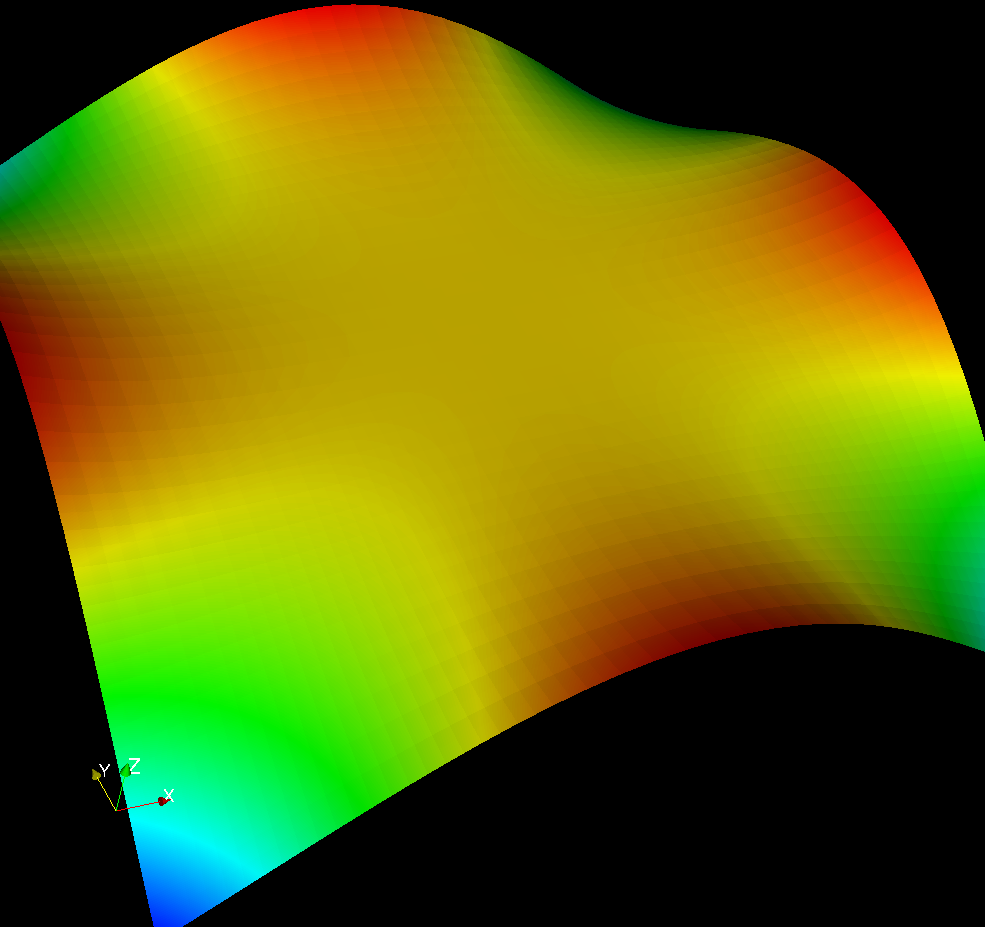
\includegraphics[width=0.49\textwidth]{./EPS/q1laplace}\hfill
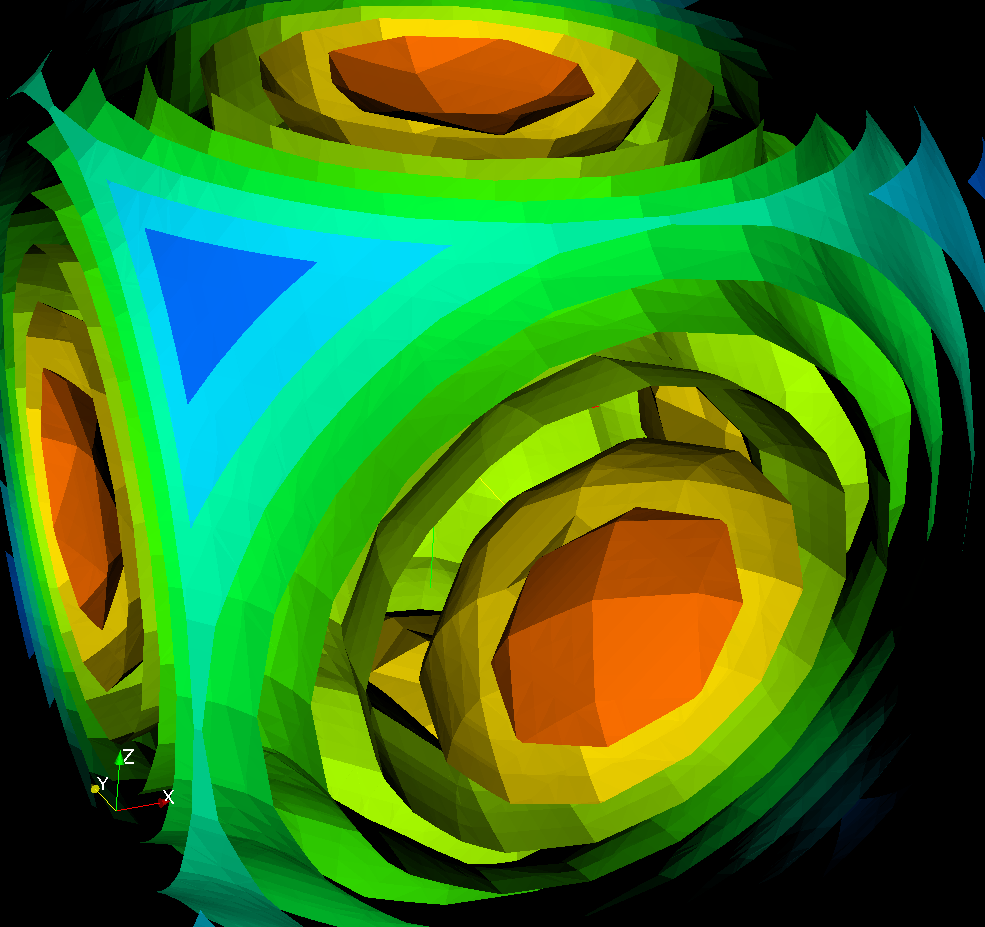
\includegraphics[width=0.49\textwidth]{./EPS/q1laplace3d}
\end{center}
\end{frame}

Figure \ref{fig:LaplaceResult} shows the output of the Laplace example
for $Q_1$ in $2d$ and $3d$. 

\mode<article>{
\begin{figure}
\begin{center}
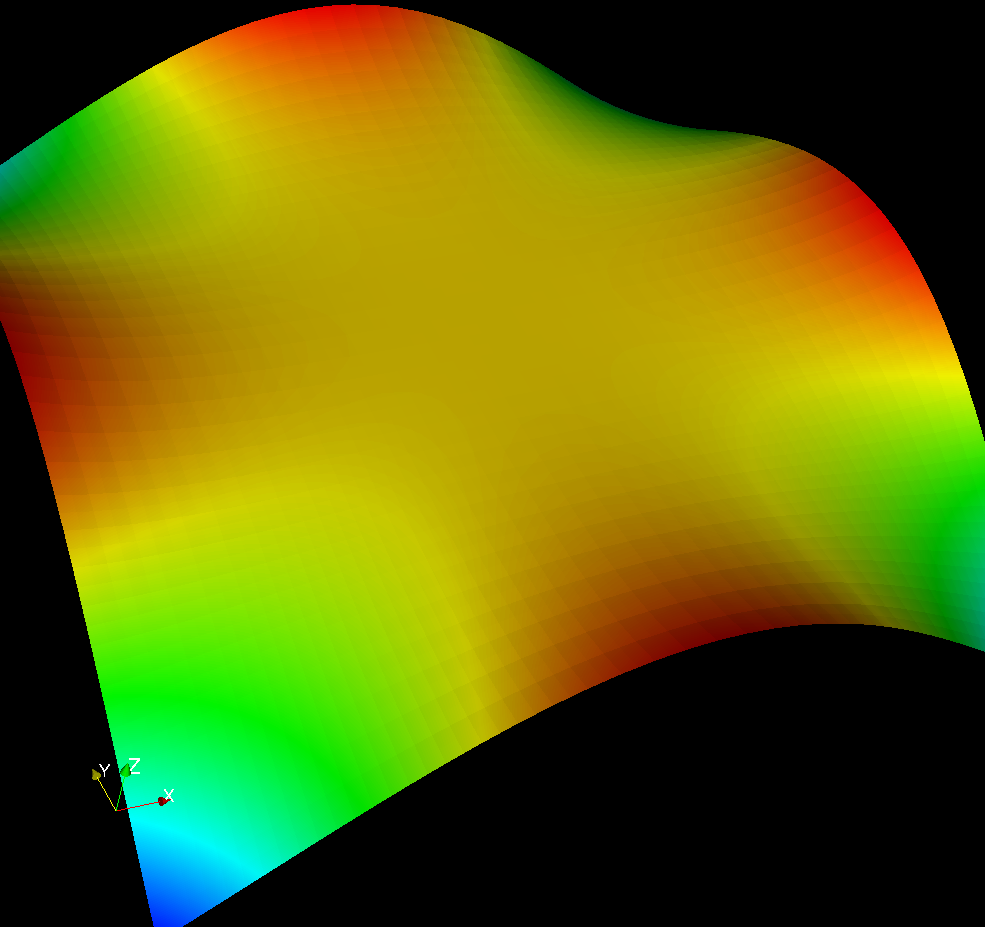
\includegraphics[width=0.49\textwidth]{./EPS/q1laplace}\hfill
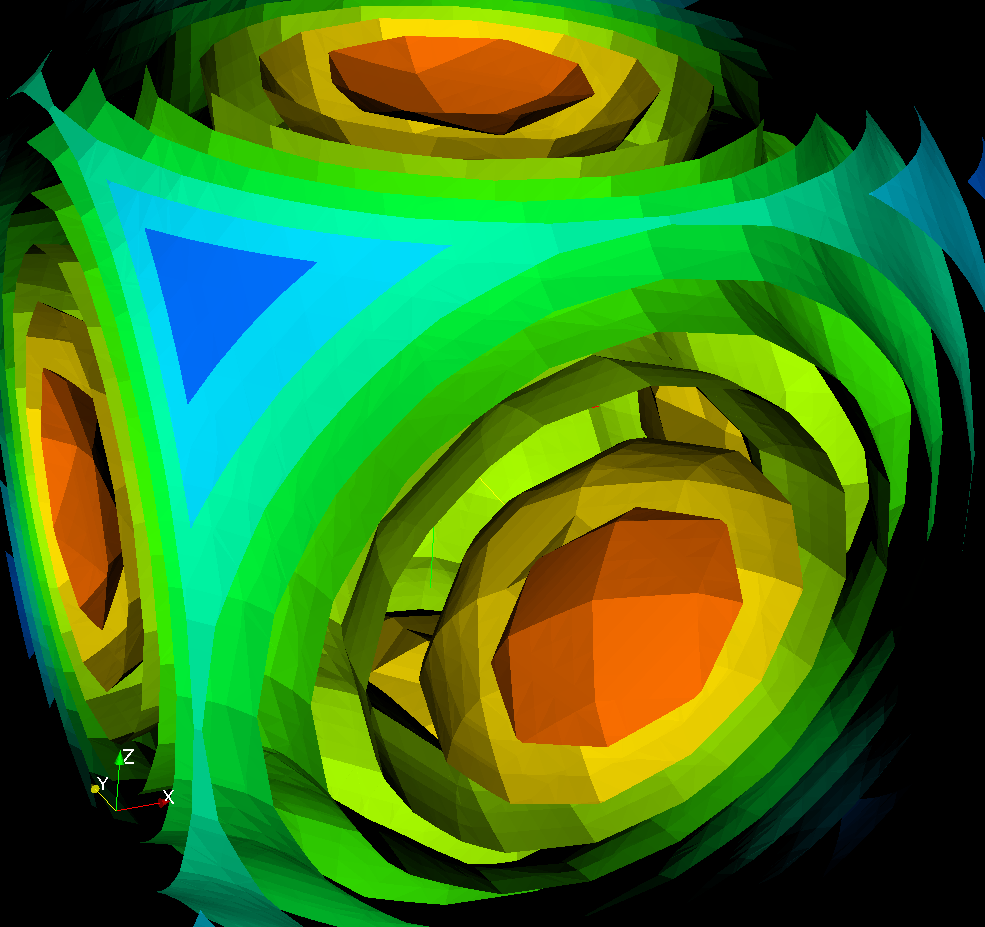
\includegraphics[width=0.49\textwidth]{./EPS/q1laplace3d}
\end{center}
\caption{Visualization of the Laplace example in $2d$ and $3d$.}
\label{fig:LaplaceResult}
\end{figure}
}

Here are some code metrix to show how much work it is to implement
various components.

\begin{frame}
\frametitle<presentation>{Some Code Metrics}
\begin{itemize}
\item Function spaces
\begin{itemize}
\item $Q_1$, $d=2$ : 80 lines + 20 lines for Dirichlet constraints.
\item $P_k$, $d=2$, $k$ a template parameter : 358 lines.
\item RT$_0$, $d=2$ : 187 lines.
\end{itemize}
\item Operators
\begin{itemize}
\item Laplace equation, Dirichlet b.c., conforming (any $d$, any $p$) : 79 lines.
\item Laplace equation, Dirichlet b.c., cell-centered FV (any $d$) : 138 lines.
\item Poisson equation, Dirichlet and Neumann b.c., conforming (any $d$, any $p$) : 196 lines.
\item Poisson equation, Dirichlet and Neumann b.c., $H(\text{div})$
conforming (mixed) method (any $d$, any $p$) : 267 lines. 
\end{itemize}
\end{itemize}
\end{frame}

And finally some computation times for various methods.

\begin{frame}
\frametitle<presentation>{Masters of the Unit Square}
Solve $-\Delta u = 0$ in $\Omega=(0,1)^2$, $u=g$ on $\partial\Omega$, $\mathcal{I}_{U_h}=10^6$, time in $s$.

\vspace{-4mm}
\begin{center} \small
\begin{tabular}{|l||r|r|r|r|}
\hline
Grid & GFS setup & Matrix setup & $\nabla\mathcal{R}$ eval. & $\mathcal{R}$ eval.\\
\hline
\multicolumn{5}{|c|}{Bilinear ($Q_1$) finite elements}\\
\hline
YaspGrid & 0.38 & 4.1 & 6.6 & 1.9 \\
UGGrid   & 0.94 & 4.8 & 9.0 & 2.5 \\
\hline
\multicolumn{5}{|c|}{Cell-centered finite volumes}\\
\hline
YaspGrid & 0.23 & 3.7 & 4.6 & 2.5 \\
UGGrid   & 0.58 & 5.2 &13.3 & 6.8 \\
\hline
\multicolumn{5}{|c|}{Linear ($P_1$) finite elements}\\
\hline
UGGrid      & 1.42 & 5.7 & 7.2 & 2.6 \\
AlbertaGrid & 1.90 & 6.2 & 6.1 & 3.0 \\
ALUGrid     & 1.78 & 6.0 & 6.0 & 2.8 \\
\hline
\multicolumn{5}{|c|}{Quartic ($P_4$) finite elements}\\
\hline
UGGrid      & 0.33 & 9.3 & 73.1 & 5.1 \\
AlbertaGrid & 0.34 & 9.3 & 77.6 & 4.9 \\
ALUGrid     & 0.31 & 9.0 & 72.0 & 4.9 \\
\hline
\end{tabular}
\end{center}

\end{frame}


\subsection{Summary}

\begin{frame}
\frametitle<presentation>{Operator Summary}
In order to implement a discretization in PDELab You have to do the
following:
\begin{itemize}
\item Write your problem in residual based form and decide which
integrals contribute to each of the volume, skeleton and boundary
terms.
\item Implement a local residual class containing:
\begin{itemize}
\item Sparsity pattern definition methods for volume/skeleton (default
versions provided, only required if matrix is assembled).
\item Residual evaluation for volume/skeleton/boundary contributions.
\item Jacobian evaluation (default with numerical differentiation
provided).
\item Jacobian application (default with numerical differentiation
provided).
\item Jacobians must be implemented, if numerical evaluation is not
desired or approximations (``Picard'') are required.
\item In the linear case, implementation of Jacobian (``local stiffness
matrix'') and default implementation of residual evaluation is more
efficient. 
\end{itemize}
\item Put everything into a grid operator space.
\end{itemize}
\end{frame}

\begin{frame}
\frametitle<presentation>{Final Notes}
Things that are still to do:
\begin{itemize}
\item Implementation of constraints (only Dirichlet is done so far,
the transformation matrices can be assembled but not applied). 
\item Newton and time-stepping schemes.
\item Real applications.
\end{itemize}

\medskip
\begin{center}
\textbf{Acknowledgements}

BMBF Project AdaptHydroMod F�rderkennzeichen 03BAPAF2

StatoilHydro Research
\end{center}
\end{frame}

\cleardoublepage
